%%____________________________________________________________________________||
\section{Simplified likelihood}
\label{sec:simplified-likelihood}

While several methods for extracting 
limits are used, the most common approach follows the frequentist paradigm using the procedure 
described in Refs.~\cite{Chatrchyan:2012tx} and ~\cite{CMS-NOTE-2011-005}. 
The observed data are interpreted using a likelihood defined as,

\begin{equation}
 \mathcal{L}(\mu, \boldsymbol{\theta}) = 
 \mathcal{P}(\mathrm{data}|\mu\cdot s(\boldsymbol{\theta}) + b(\boldsymbol{\theta})) \cdot p(\tilde{\boldsymbol{\theta}}|\boldsymbol{\theta})
\label{eq:generic-likelihood}
\end{equation}

where $\mathcal{P}(\mathrm{data}|\mu\cdot s(\boldsymbol{\theta}) + b(\boldsymbol{\theta}))$ is a product of the probability 
over all events or bins in one or more discriminating variables or event categories to observe the data. The parameters 
$\boldsymbol{\theta}=\left(\theta_{1},\theta_{2}...\right)$ are nuisance parameters, which are used to model the variation of the 
signal $s(\boldsymbol{\theta})$ and background $b(\boldsymbol{\theta})$ models due to systematic uncertainties. Often, these nuisance 
parameters are constrained by external measurements, $\tilde{\boldsymbol{\theta}}$, which are encoded in the 
probability density function $p(\tilde{\boldsymbol{\theta}}|\boldsymbol{\theta})$. 
The parameter $\mu$, typically referred to as a signal strength, is a common scale factor for the expected signal contribution. 
A particular BSM model predicting $s(\boldsymbol{\theta})$ is said to be excluded at some confidence level 
when every value of $\mu\ge1$ is excluded at at least that confidence level.

In order to achieve a good sensitivity to a wide range of BSM models, searches are often performed 
by categorising events with different final states or according to some discriminating variable. 
The precise modelling of the backgrounds can therefore be rather complicated, involving many 
nuisance parameters. For this reason, the full likelihood is therefore often 
too detailed to describe in a CMS publication and includes too many (nuisance) parameters to provide numerically. 
The following describes a procedure for using a reduced set of information provided by the CMS Collaboration to 
re-interpret searches for new physics through the use of a simplified likelihood. 


\subsection{Defining the simplified likelihood}
In practise, the likelihood defined in Equation~\ref{eq:generic-likelihood} can include regions in which negligible signal is expected under a wide 
range of BSM models. Typically these are referred to as ``control'' regions in that they allow to constrain the nuisance parameters that  
cause large variations in the background model.
In this note, the distinction is made between these regions and ``search'' regions, which instead 
are expected to include contributions from the signal, under some particular set of BSM models. A search region 
is defined by a set of criteria used to select events. These criteria can include categorisations based on 
the number of a certain type of object in the event such as jets or 
charged leptons, and intervals in some discriminating variable such as the missing transverse momentum in the event. The data in each search region, $i$, is characterised 
by a single number, $n_{i}$ which is the observed number of events. The likelihood is therefore constructed from a product of counting 
experiments, representing each search region in one or more search regions. 
For a given search region, $i$, the probability to observe $n_{i}$ events is given by

\begin{equation}
 P(n_{i}|\mu \cdot s_{i}+b_{i}) = \dfrac{(\mu \cdot s_{i}+b_{i})^{n_{i}} e^{-(\mu \cdot s_{i}+b_{i})} }{n_{i}!}
\label{eq:poisson-likelihood}
\end{equation}

where $s_{i}$ and $b_{i}$ are the total expected signal and background contributions.\footnote{In the case 
that the search region $R_{i}$ is a bin or interval in a distribution of some observable $x$, for which the signal and background models $s(x)$ 
and $b(x)$ are continuous functions of $x$ the values of $s_{i}$ and $b_{i}$ are taken as 
$s_{i}=\int_{R_{i}} s(x)dx$ and $b_{i}=\int_{R_{i}} b(x)dx$.}

In most cases, the background contribution in each search region will not be known with perfect accuracy and is therefore 
subject to systematic uncertainties. These uncertainties are modelled by modifying the background contributions as 
$b_{i}\rightarrow b_{i}+\theta_{i}$. 
The probability to simultaneously observe each of the $n_{i}$ events in $N$ search regions is the product of probabilities across the search regions such that,

\begin{equation}
\mathcal{P}(\mathrm{data}|\mu\cdot s(\boldsymbol{\theta}) + b(\boldsymbol{\theta})) = \prod_{i=1}^{N} P(n_{i}|\mu \cdot s_{i}+b_{i}+\theta_{i})
\label{eq:poisson-prob}
\end{equation}

Some simplifying assumptions must be made in order to avoid the necessity to publish the full probability density function $p(\tilde{\boldsymbol{\theta}}|\boldsymbol{\theta})$. 

\begin{itemize}
\item{The constraints on the background contributions are Gaussian such that the distribution of the number of background events is symmetric about the expectation, $b_{i}$, 
and its variance is independent of $\boldsymbol{\theta}$. Often, the background contributions are estimated from control regions in data with large sample sizes, which allows for this 
assumption to be made.}

\item{The covariance, and therefore only the linear correlation, between the background contribution in each region is enough to approximate $p(\tilde{\boldsymbol{\theta}}|\boldsymbol{\theta})$ 
at least for values of $\boldsymbol{\theta}$ which are close to $\tilde{\boldsymbol{\theta}}$.}

\item{The number of events $n_{i}$ are statistically independent from one another and the background contributions $b_{i}$ and covariance matrix $\mathrm{\mathbf{V}}$ are 
statistically independent of the data from all search regions. This is true when there are no events which are included in more than one search region and when the methods used to 
determine $b_{i}$ and $\mathrm{\mathbf{V}}$ do not use the data from the search regions.}

\item{The systematic uncertainties in the signal can be neglected. These will strongly depend on the specific BSM physics model. 
Systematic uncertainties on the signal can be accounted for by adding appropriate nuisance parameters with Gaussian constraints 
as for the background contributions. }
\end{itemize}

Under these assumptions, $p(\tilde{\boldsymbol{\theta}}|\boldsymbol{\theta})$ can be modelled as a multivariate Gaussian with the mean vector identified with external measurements of 
$\tilde{\boldsymbol{\theta}}=0$. The simplified likelihood can now be expressed as,

\begin{equation}
\mathcal{L}_{S}(\mu, \boldsymbol{\theta}) =  \prod_{i=1}^{N} \dfrac{(\mu \cdot s_{i}+b_{i}+\theta_{i})^{n_{i}} e^{-(\mu \cdot s_{i}+b_{i}+\theta_{i})} }{n_{i}!} \cdot  
\mathrm{exp}\left(-\dfrac{1}{2} \boldsymbol{\theta}^{T}\mathrm{\mathbf{V}}^{-1}\boldsymbol{\theta} \right)
\label{eq:full-likelihood}
\end{equation}

where $\mathrm{\mathbf{V}}$ represents the covariance matrix for the expected background contributions across the search regions.
In the following example, the simplfied likelihood is constructed using the statistics package {\sc RooFit}~\cite{roofit} but it should be noted that 
the procedure does not prohibit the use of any other tool for its construction. 

\subsection{Example of constructing the simplified likelihood}
\label{sec:sl-toy}

A toy example of a search for BSM physics is represented in Figure~\ref{fig:toy-example}. The search is performed using 8 mutually exclusive search regions 
which vary in the expected contributions from backgrounds and a potential BSM physics signal. The backgrounds of this search are $\mathrm{Z+jets}$ and $\mathrm{W+jets}$ processes in which the 
W or Z boson decays to final states with a neutrino, which are commonly the dominant sources of backgrounds in searches for BSM physics. Figure~\ref{fig:toy-example} (a) indicates the 
number of observed events in each of the search regions as well as the expected contribution from the two different sources of background, stacked on top of one another. 
The background estimates include systematic uncertainties related to theoretical uncertainties, when the backgrounds are derived using 
simulation, and experimental uncertainties related to the resolutions and response of the detector. They can also include a statistical component 
due to limited sample sizes of events in control regions used to estimate the backgrounds. In this example, two systematics are included, one affecting the $\mathrm{Z}(\rightarrow \nu\nu)+\mathrm{jets}$ background only
and one affecting the $\mathrm{W}(\rightarrow l\nu)+\mathrm{jets}$ background only. These two systematics are modelled as two nuisance parameters in the full likelihood of Equation~\ref{eq:generic-likelihood}. 
Figure~\ref{fig:toy-example} (b) shows the variation of the expected contribution due to the systematic uncertainties. 
The dot and dot--dashed histograms show the expected 
contributions when each of the two nuisance parameters are varied positively and negatively, respectively.
Finally, the expected contribution from a BSM physics signal is shown. 
The ratio of the expected signal to the total background estimate in each region is shown in the lower panel of Figure~\ref{fig:toy-example} (b). 
In this example, the signal is provided, however, the 
signal can be exchanged for some other BSM physics process using a number of publicly available event generators and tools that simulate the response 
and resolution of the CMS detector. The details of producing signal estimates is beyond the scope of this note. 

\begin{figure}[hbt]
  \begin{center} 
   \subfloat[][]{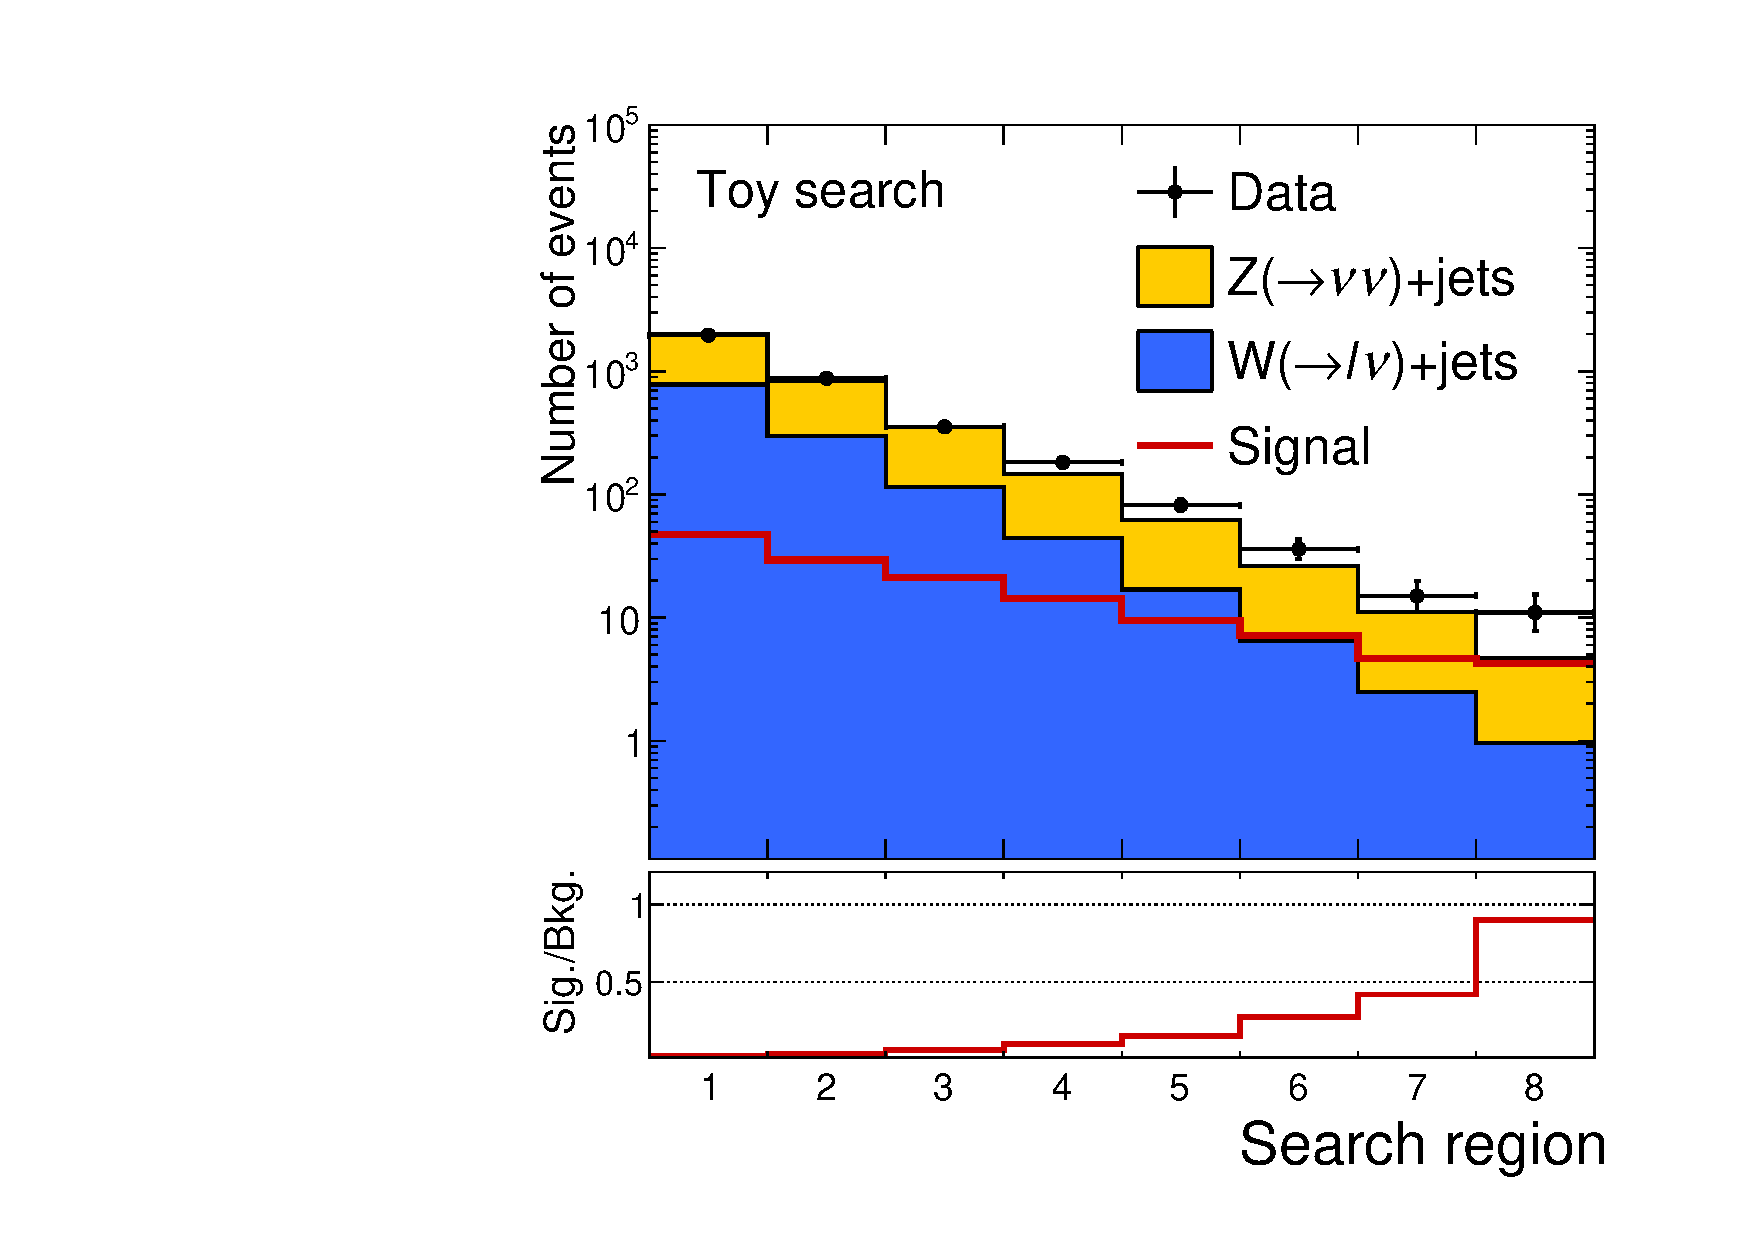
\includegraphics[width=1.2\cmsFigWidth]{figures/plot_dummy.pdf}}
   \subfloat[][]{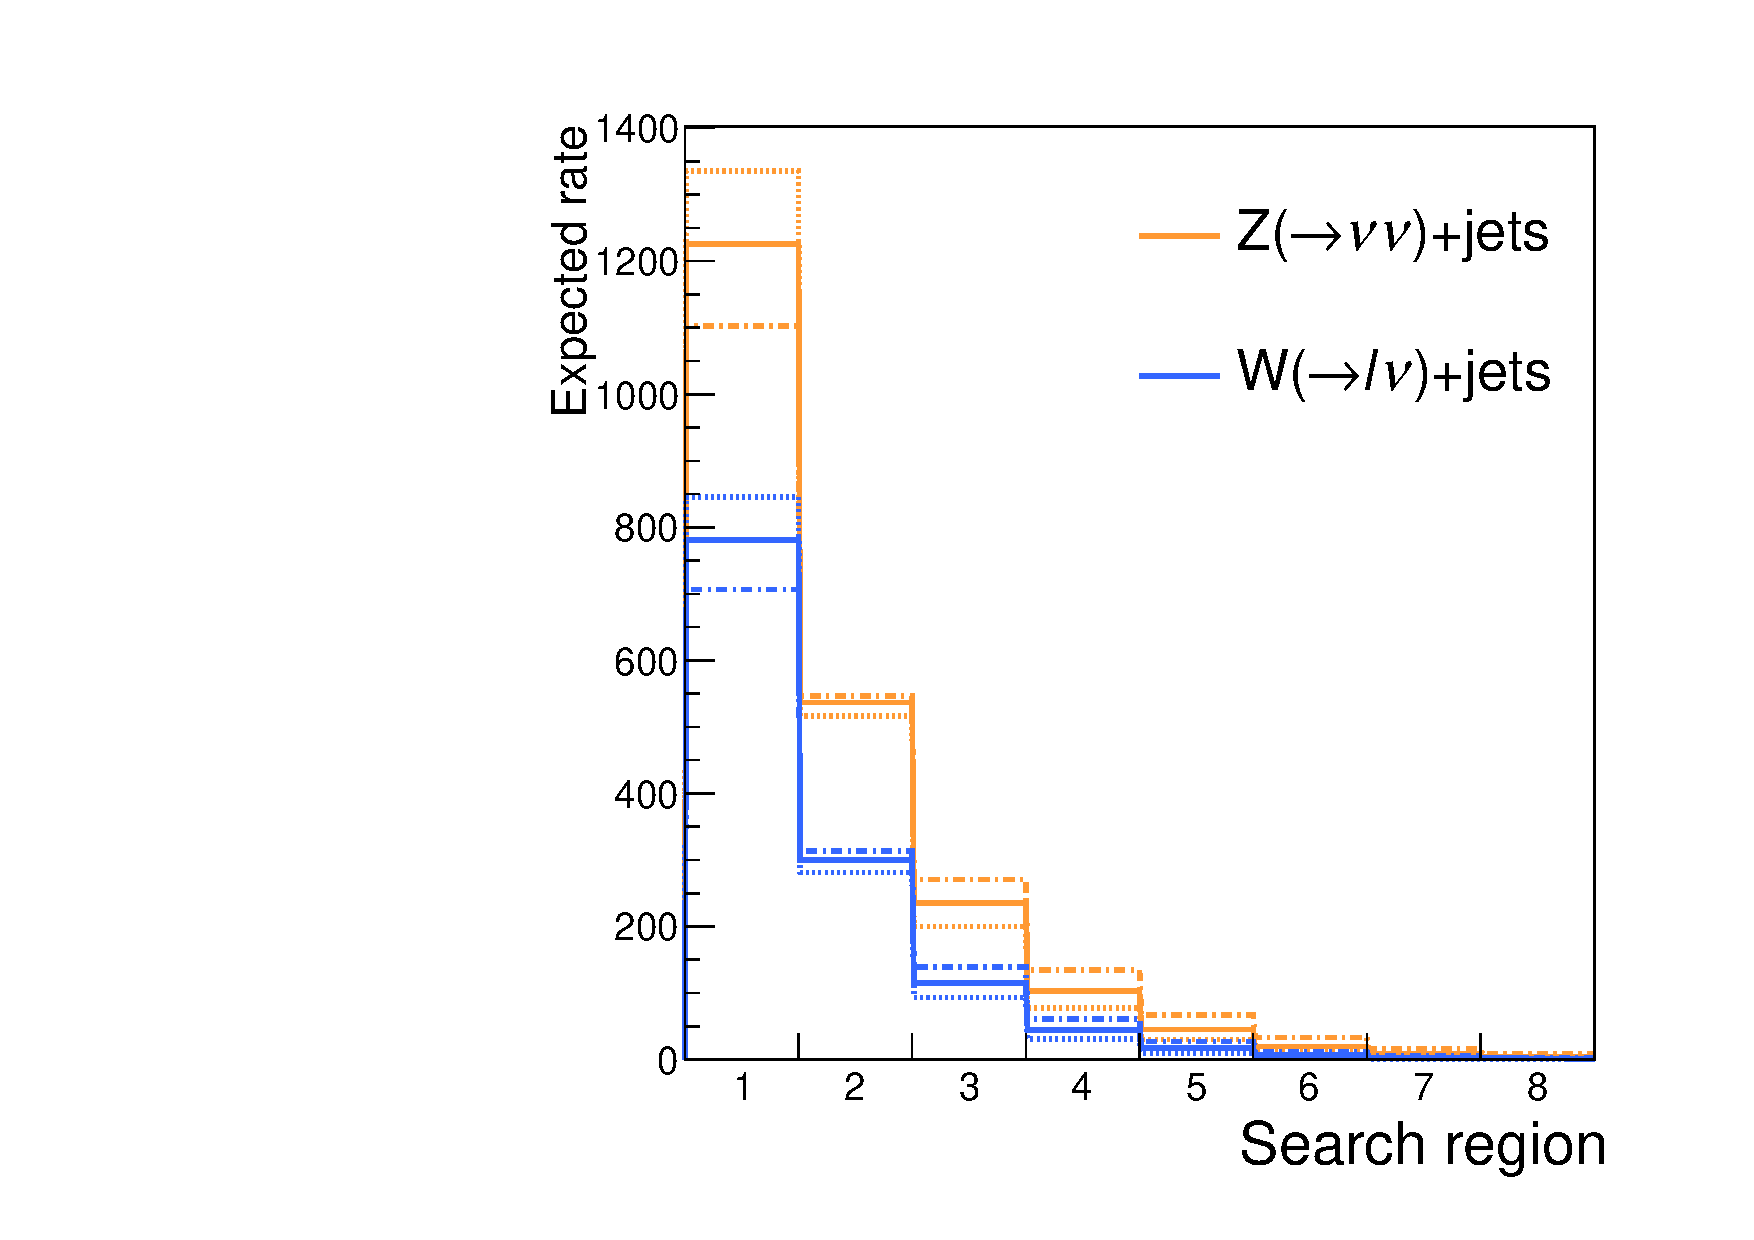
\includegraphics[width=1.2\cmsFigWidth]{figures/systematics.pdf}}
   \caption{(a) Number of data, expected background and expected signal in the 8 search regions. The lower panel shows the ratio of the expected signal to the total expected background. 
(b) Uncertainties in the two background contributions. The dotted and dot--dashed lines show the expected number of background events in each process when shifting the systematic uncertainty to positive values and negative values respectively.}
   \label{fig:toy-example} 
  \end{center}
\end{figure}

The relevant information in the toy search for the simplified likelihood construction is summarised in Table~\ref{tab:toytable}.
Furthermore, Figure~\ref{fig:covariance} gives the covariance between the total rate of 
background contributions expected in each of the search regions. The non-zero off-diagonal values are a result of the fact that the estimate of the 
backgrounds are not independent in each region since the systematic effects cause correlated variations of the expected contributions of the two backgrounds 
across the regions. 

\begin{table}[!htb]
\caption{Observed number of events and total expected background and signal rates for each of the 8 search regions.}
 \begin{center}
 \begin{tabular}{|c|c|c|c|}
\hline
Search region ($i$) & Data ($n_{i}$) & Total background ($b_{i}$) & Signal ($s_{i}$) \\
\hline
1 & 1964 & 2006.4 & 47.0 \\
2 & 877 & 836.4 & 29.4 \\
3 & 354 & 350.0 & 21.1 \\
4 & 182 & 147.1 & 14.3 \\
5 & 82  & 62.0  & 9.4 \\
6 & 36  & 26.2  & 7.1 \\
7 & 15  & 11.1  & 4.7 \\
8 & 11  & 4.7   & 4.3 \\
\hline
\end{tabular}
\end{center}
\label{tab:toytable}
\end{table}

\begin{figure}[hbt]
  \begin{center} 
   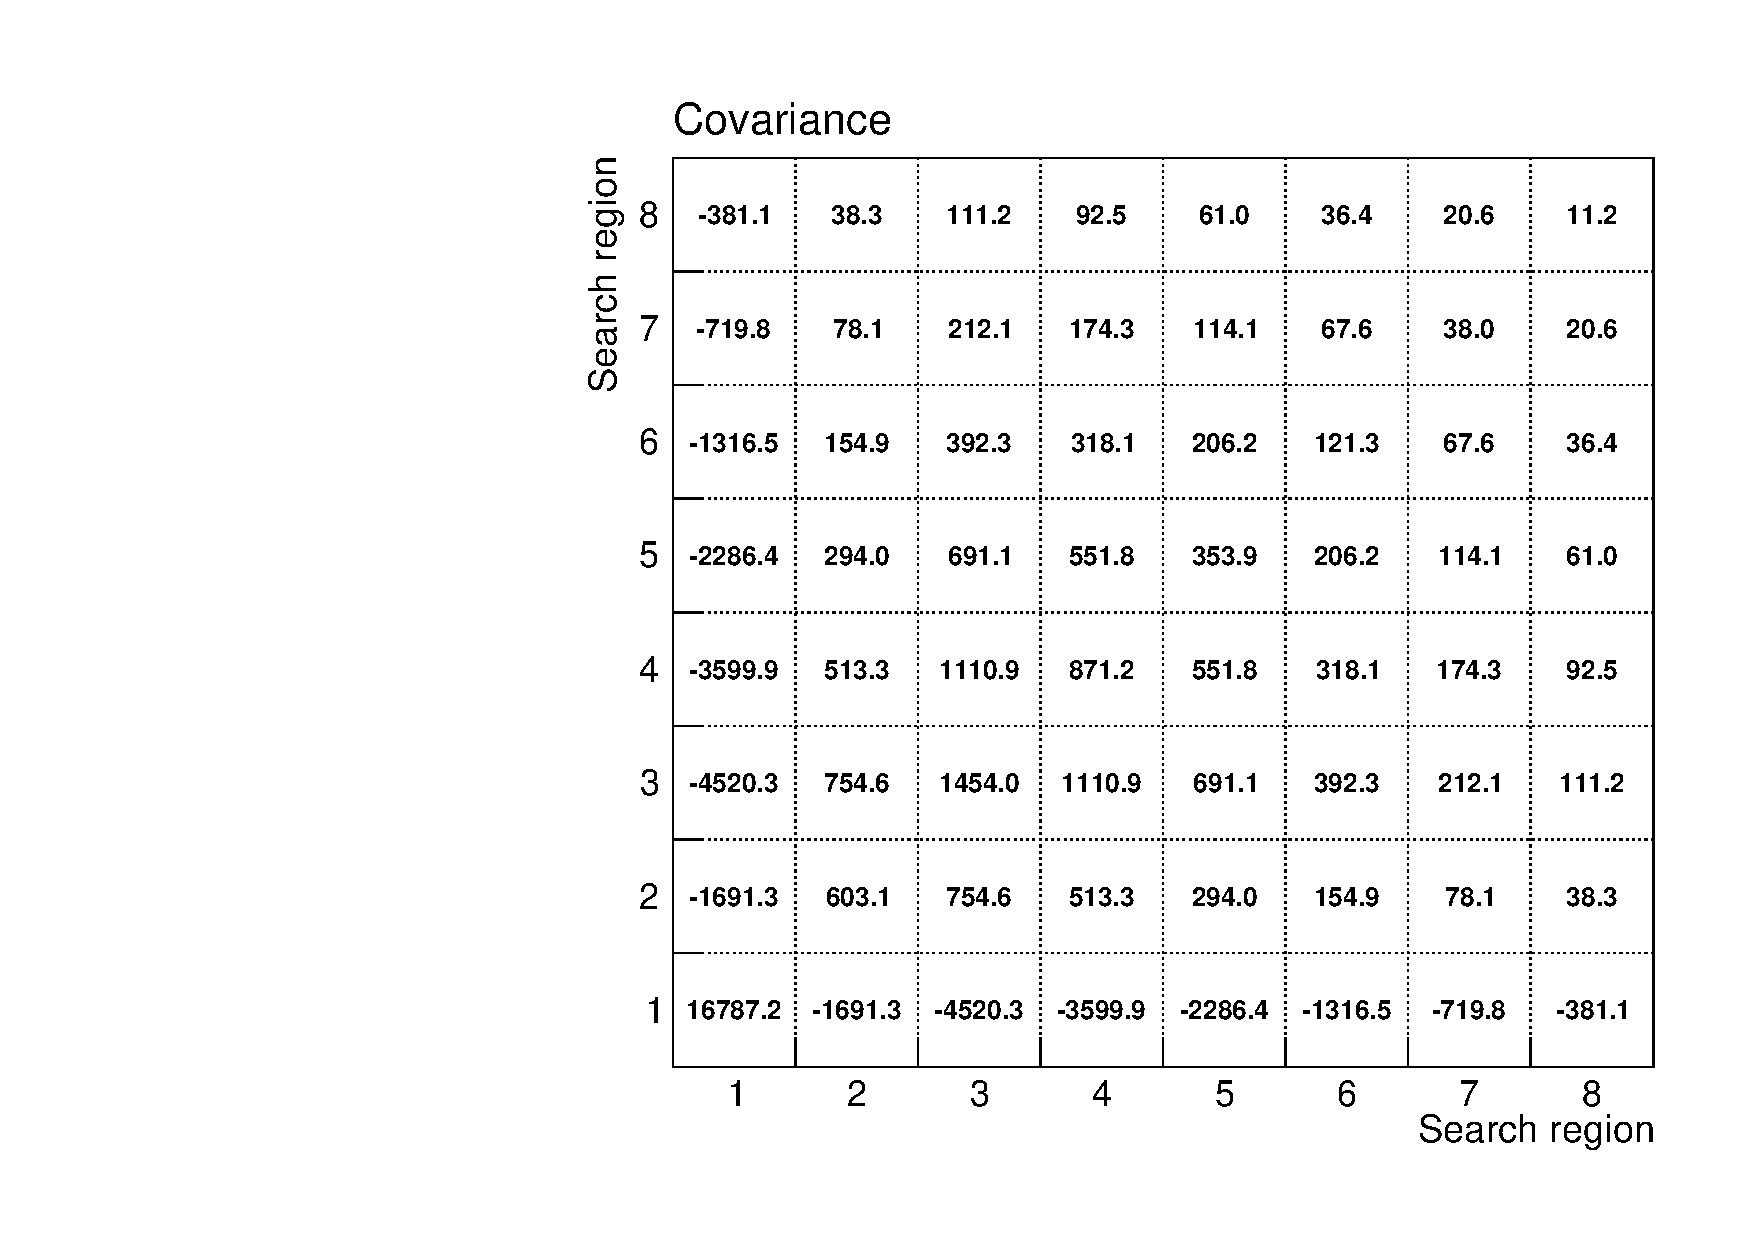
\includegraphics[width=1.8\cmsFigWidth]{figures/htsearch_covariance.pdf}
   \caption{Covariance between the total rate of background  contributions expected  in each of the  search regions.}
   \label{fig:covariance} 
  \end{center}
\end{figure}

The information provided in Table~\ref{tab:toytable} and Figure~\ref{fig:covariance} is all that is necessary to reconstruct the likelihood in Equation~\ref{eq:full-likelihood} and 
can be summarised as follows; 

\begin{itemize}
\item {The number of observed events in each search region, $n_{i}$.}
\item {The background and signal expectations in each search region, $b_{i}$ and $s_{i}$.}
\item {The covariance between the number of background events in each search region, $\mathrm{\mathbf{V}}=\left\{V_{ij}\right\}_{i,j=1}^{8}$. }
\end{itemize}

It is important to note that the estimates of both the background contributions and the 
covariance matrix do not use the data in the 8 search regions, making them statistically independent from the data. The data in the search regions 
can be used to further constrain the background (meaning to reduce the uncertainties on the nuisance parameters $\boldsymbol{\theta}$) through the use 
of the profiled likelihood ratio, which is defined as 

\begin{equation}
q(\mu) = -2\ln \dfrac {\mathcal{L}_{S}(\mu,\hat{\boldsymbol{\theta}}_{\mu})} {\mathcal{L}_{S}(\hat{\mu},\hat{\hat{\boldsymbol{\theta}}})}
\label{eq:llr}
\end{equation}

where $\hat{\mu}$ and $\hat{\hat{\boldsymbol{\theta}}}$ are the values of the parameters $\mu$ and $\boldsymbol{\theta}$ respectively, 
which maximise the likelihood. The values $\hat{\boldsymbol{\theta}}_{\mu}$ are the values of $\boldsymbol{\theta}$ which maximise the 
likelihood for a fixed value of $\mu$. The value of $\hat{\mu}$ is usually referred to as the ``best-fit'' value.

A common estimate of the uncertainty in $\mu$ is to determine the interval in $\mu$ such that $q(\mu)\leq1$ and define the uncertainty as the difference between 
the end points of that interval and $\hat{\mu}$. Furthermore, the profiled likelihood is a common tool when defining test statistics for setting limits and quantifying excesses 
in BSM searches performed by the CMS collaboration, a full description of which can be found in Refs.~\cite{Chatrchyan:2012tx}. The 
uncertainty in $\mu$ often provides a good indication of the sensitivity of a search to a given BSM signal. 

Figure~\ref{fig:likelihoodscan} shows the value of $q(\mu)$ as a function of $\mu$. The values when $q(\mu)$ 
is defined using the likelihood of Equation~\ref{eq:full-likelihood} are shown and compared with the same definition but assuming no correlations between the 
background yields by setting $V_{ij}=0$ for $i\neq j$. The results substituting $\mathcal{L}_{S}\rightarrow\mathcal{L}$ in Equation~\ref{eq:llr}, 
namely using the full likelihood of Equation~\ref{eq:generic-likelihood}, are also shown.The simplified 
likelihood provides shows good agreement with the full likelihood while it is clear that ignoring the correlations results in a bias of the estimate of $\hat{\mu}$. In 
addition, the width of the curve ignoring the correlation is larger than the other curves meaning the uncertainty estimate on $\mu$ will be overestimated.  


\begin{figure}[hbt]
  \begin{center} 
   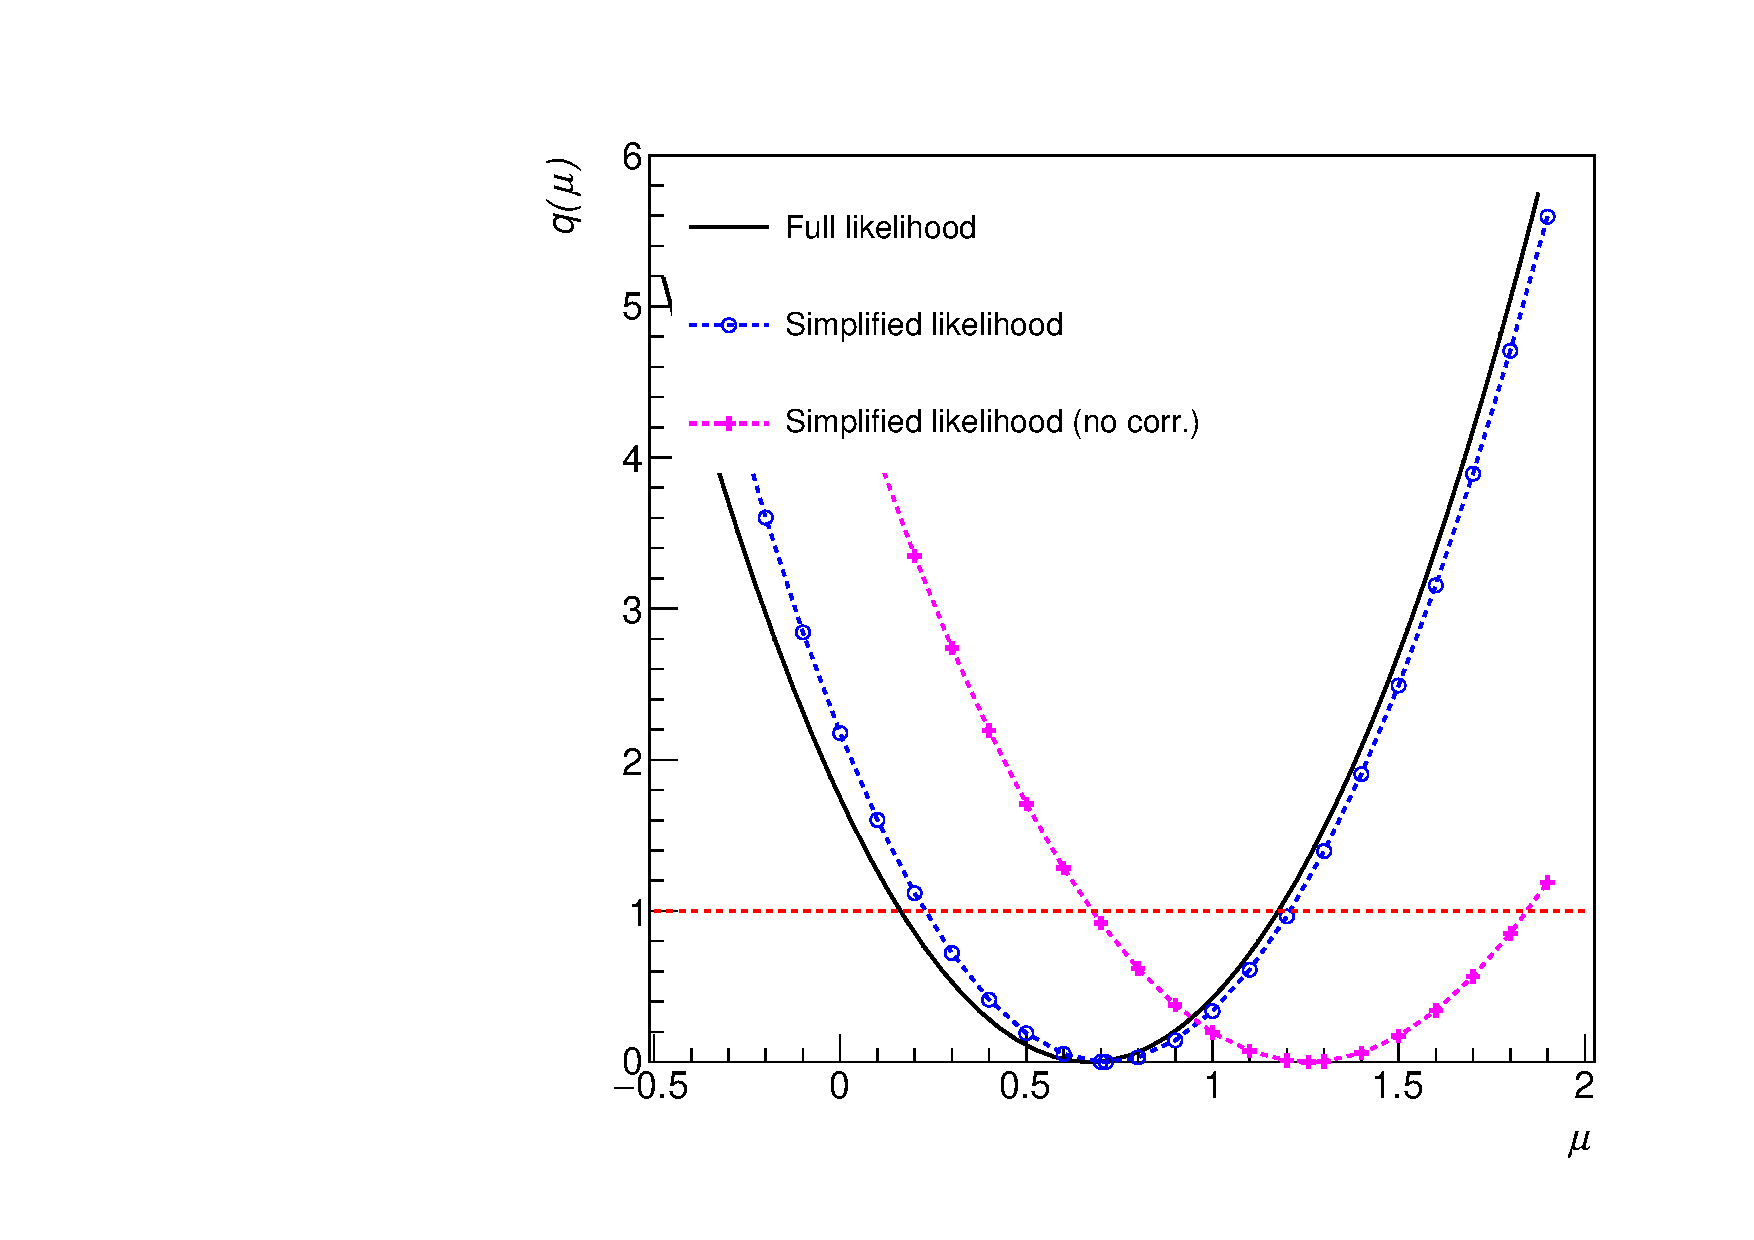
\includegraphics[width=1.5\cmsFigWidth]{figures/r.pdf}
   \caption{The value of $q(\mu)$ defined using the simplified likelihood using the full covariance matrix (open blue points), assuming no correlations between the 
   background yields (open magenta crosses) and defined using the full likelihood (solid black line).}
   \label{fig:likelihoodscan} 
  \end{center}
\end{figure}


% covariance must be taken as the result of a maximum likelihood fit considering the control regions only. 
% If the control region is not included then the results fit may be taken. 
%%____________________________________________________________________________||
% \subsection{Motivation}
% \begin{itemize}
% \item Even with SSR recasters have insufficient information to reproduce analysis
% \item Full likelihood is overkill - what is necessary?
% \end{itemize}
% \subsection{Theory}
% \label{sec:sl-theory}
% \begin{itemize}
% \item Definition of simplified likelihood
% \item Inputs needed
% \item What's simplified? No signal systs, no CR, gaussian unc
% \end{itemize}
% \subsection{Procedure}
% \label{sec:sl-procedure}
% \begin{itemize}
% \item Determining correlation matrix
% \item Defining likelihood
% \item For study of impact setting off-diag elements to 0
% \end{itemize}
% \subsection{Signal contamination}
% \label{sec:signal-contamination}
% \begin{itemize}
% \item Definition of reduced efficiency method
% \item What do recasters need to take account of contamination?
% \end{itemize}
% \subsection{Results}
% \begin{itemize}
% \item Covariance matrix
% \item DeltaNLL vs r for example model (compare with + without correlations)
% \item Limit planes for several models (T1qqqq, T2tt, T2bb)
% \item Ratios + comparison to full
% \end{itemize}
